\documentclass{article}

\PassOptionsToPackage{numbers, compress}{natbib}

% TODO: Reformat paper before submission, make sure the formatting is proper

% ready for submission
%     \usepackage{neurips_2021}
% to compile a camera-ready version, add the [final]

% remove this before submission
\usepackage{lineno}
\linenumbers%

\usepackage[final]{neurips_2021}
\usepackage{booktabs}       % professional-quality tables
\usepackage{pgfplotstable}  % read csv tables
\pgfplotsset{compat=1.14}
\usepackage{longtable}

\usepackage[utf8]{inputenc} % allow utf-8 input
\usepackage[T1]{fontenc}    % use 8-bit T1 fonts
\usepackage{hyperref}       % hyperlinks
\usepackage{url}            % simple URL typesetting
\usepackage{amsfonts}       % blackboard math symbols
\usepackage{nicefrac}       % compact symbols for 1/2, etc.
\usepackage{microtype}      % microtypography
\usepackage{xcolor}         % colors

\title{%
    S$^4$AD-Learning: Self-supervised Semi-supervised Active Deep Learning
}

\author{%
  Joao Fonseca\thanks{Correponding author.} \\
  NOVA Information Management School\\
  Universidade Nova de Lisboa\\
  \texttt{jpfonseca@novaims.unl.pt} \\
  \And%
  Fernando Bacao \\
  NOVA Information Management School\\
  Universidade Nova de Lisboa\\
  \texttt{bacao@novaims.unl.pt} \\
}

\begin{document}

\maketitle

\begin{abstract}
    TODO
\end{abstract}


\section{Introduction}~\label{sec:introduction}

This is an introduction.

Learning-based AL selection is an important yet under-explored
problem~\cite{gao2020consistency}.

The proposed method extends the model described in~\cite{bengar2021reducing}
in the following ways: (1) Add a Semi-supervised learning loss to leverage the
informativeness of both labeled and unlabeled data in the iterative process,
(2) Extend the Self-supervised Active Learning model using data augmentation
as a regularization method, (3) Combine the LADA-LearningLoss data acquisition
method proposed in~\cite{kim2021lada} with the VAAL model~\cite{kim2021task}.

\section{Background}

\subsection{Problem Formulation}

% Define the AL problem

\subsection{Data Augmentation in AL}

% Look ahead data augmentation
Data Augmentation in AL has been recently explored for different
domains~\cite{kim2021lada, quteineh2020textual, li2021framework}.
LADA~\cite{kim2021lada}. They test two data augmentation methods, one using
Spatial Transformer Networks {\bf [CITATION]}, and another using the Mixup
method.

% VAE adversarial Active Learning (2019)
The Variational Adversarial Active Learning model~\cite{sinha2019variational}

% Task-aware Variational Adversarial Active Learning (2021)
The Task-aware VAAL model~\cite{kim2021task} improves over the VAAL model
via\ldots

% Related AL data augmentation
{\bf Copy/pasted from the LADA paper:} "BayesianGenerative Active Deep Learning
(BGADL) combines acquisition and augmentation in a pipelinedapproach [11];
BGADL selects data instances viafacq, and BGADL augments the selected
instancesviafaug, which is VAE-ACGAN.  However, BGADL limits the vicinity to
preserve the label validity.Also, a large number of labeled instances are
demanded to train the generative model, VAE-ACGAN,of BGADL at every
acquisition round. More importantly, BGADL does not consider the potentialgain
from data augmentation in the process of acquisition."

\subsection{Semi-supervised Learning in AL}

Consistency-based semi-supervised active learning~\cite{gao2020consistency}.
Combining mixmatch and active learning for better accuracy with fewer
labels~\cite{song2019combining}.

% Semi-supervised Learning in AL - Which classifier should be used?
S$^4$L~\cite{zhai2019s4l} combines self-supervised and semi-supervised
learning training losses simultaneously, which assumes existence of a small
labeled training dataset.

\subsection{Self-supervised Learning in AL}

% self-supervised - simCLR
SimCLR~\cite{chen2020simple}

% self-supervised - Bootstrap your own latent (BYOL)
BYOL~\cite{grill2020bootstrap}

% self-supervised - SubTab
SubTab~\cite{ucar2021subtab}

% self-supervised in AL
Active Learning (AL) using self-supervised learning was explored
in~\cite{margatina2021active}. They used a pretrained BERT
model~\cite{devlin2019bert} with a task-specific classification layer to
natural language processing classification tasks. They proposed an Uncertainty
Criterion based on the use of the average Kullback-Leibler (KL) divergence
between an unlabeled observation $x_p$, from the unlabeled data pool
$\mathcal{D}_{pool}$, and its $k$-nearest neighbors (KNN), ${x_l^{(i)}},
i=1,\ldots,k$, from the set of labeled data $\mathcal{D}_{lab}$ in the feature
space, produced via an encoder $\Phi(\mathcal{D}_{lab})$ and
$\Phi(\mathcal{D}_{pool})$. They select $b$ observations from
$\mathcal{D}_{pool}$ with the highest average KL divergence score to be
labeled and moved into $\mathcal{D}_{lab}$ for the next AL iteration.

An earlier attempt to joining AL with self-supervised is proposed
in~\cite{yuan2020cold}.

Another method was proposed in~\cite{bengar2021reducing} 

\subsection{Active Deep Learning}

% Deep AL - general overview of literature
A literature review of Deep AL can be found in~\cite{ren2021survey}.

% Learning Loss - Compare vs KL? 
Learning Loss in AL was proposed in~\cite{yoo2019learning}, which replaces the
traditional Uncertainty Criterion module. However,
in~\cite{shukla2021mathematical}, a second iteration of this module,
LearningLoss++, improves it using a KL divergence based objective by
comparing gradients. {\bf [To be clarified later]}

% The core-set approach
The core-set model~\cite{sener2017active}

\section{Methodology}

\subsection{The S\texorpdfstring{$^4$}{TEXT}AD-Learning Model}

\begin{figure}[htb]
	\centering
    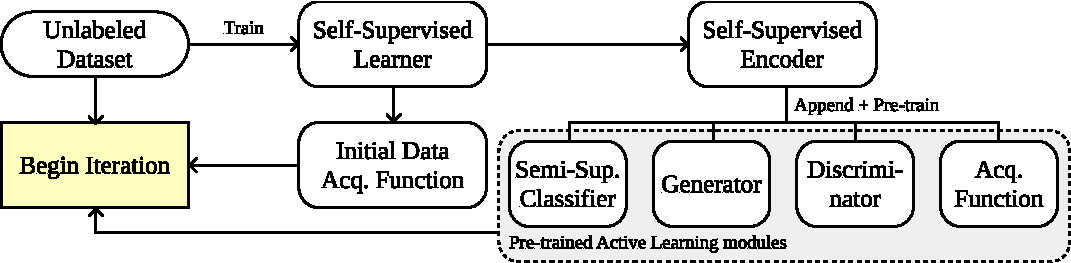
\includegraphics[width=\linewidth]{../analysis/al_initialization}
    \caption{%
        Diagram depicting the initialization of the proposed model. 
    }~\label{fig:al_initialization}
\end{figure}

\begin{figure}[htb]
	\centering
    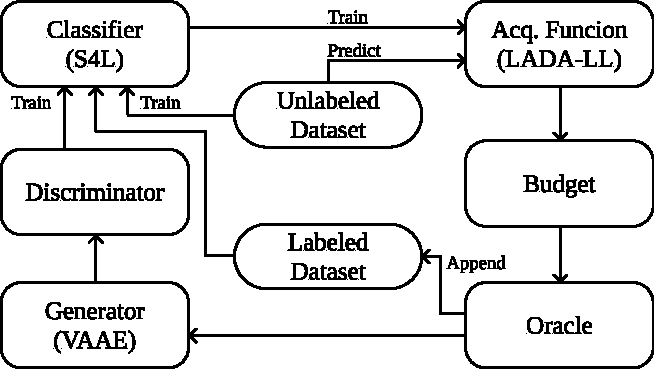
\includegraphics[width=.6\linewidth]{../analysis/al_iteration}
    \caption{%
        Diagram depicting the iterative procedure of the proposed model. 
    }~\label{fig:al_iteration}
\end{figure}

\subsection{Self-supervised initialization}

\subsubsection{Initial Data Acquisition Function (TBD)}

\subsubsection{Pseudo-labeling fine tuning}

\subsection{Integrated Augmentation and Acquisition}

\subsubsection{Variational Adversarial Autoencoder}

\subsubsection{Look-Ahead Data Acquisition with LearningLoss++}

\section{Experiments}

\subsection{Baselines and Datasets}

Datasets planned for use:

\begin{itemize}
    \item CIFAR-10
    \item CIFAR-100
    \item FashionMNIST
    \item SVHN
\end{itemize}

% \begin{table}
%     \centering
%     \caption{\label{tab:datasets_description}
%         Description of the datasets collected after data preprocessing. The
%         sampling strategy is similar across datasets. Legend: (IR) Imbalance
%         Ratio
%     }
%     \pgfplotstabletypeset[
%         col sep=comma,
%         string type,
%         every head row/.style={%
%             before row=\toprule,
%             after row=\midrule
%         },
%         every last row/.style={after row=\bottomrule},
%     ]{../analysis/datasets_description.csv}
% \end{table}

Baseline models planned for use:

\begin{itemize}
    \item Random
    \item Coreset
    \item LearningLoss++
    \item LADA
    \item CAL (Contrastive Active Learning)
    \item BALD
\end{itemize}

\subsection{Quantitative Performance Evaluations}

% Also add here an analysis of semi-supervised performance of the proposed
% model

\subsection{Qualitative Analysis on Acquired Data Instances}

\section{Conclusions}

\section{Broader Impact}

\section{Acknowledgements}

\bibliography{references}
\bibliographystyle{ieeetr}

\section*{Checklist}

The checklist follows the references. Please read the checklist guidelines
carefully for information on how to answer these questions. For each
question, change the default \answerTODO{} to \answerYes{}, \answerNo{}, or
\answerNA{}. You are strongly encouraged to include a {\bf justification to
your answer}, either by referencing the appropriate section of your paper or
providing a brief inline description. For example:
\begin{itemize}
  \item Did you include the license to the code and datasets? \answerYes{See
      Section~\ref{sec:introduction}.}
  \item Did you include the license to the code and datasets? \answerNo{The
      code and the data are proprietary.}
  \item Did you include the license to the code and datasets? \answerNA{}
\end{itemize}

Please do not modify the questions and only use the provided macros for your
answers. Note that the Checklist section does not count towards the page
limit. In your paper, please delete this instructions block and only keep the
Checklist section heading above along with the questions/answers below.

\begin{enumerate}

\item For all authors\ldots
\begin{enumerate}
  \item Do the main claims made in the abstract and introduction accurately reflect the paper's contributions and scope?
    \answerTODO{}
  \item Did you describe the limitations of your work?
    \answerTODO{}
  \item Did you discuss any potential negative societal impacts of your work?
    \answerTODO{}
  \item Have you read the ethics review guidelines and ensured that your paper conforms to them?
    \answerTODO{}
\end{enumerate}

\item If you are including theoretical results\ldots
\begin{enumerate}
  \item Did you state the full set of assumptions of all theoretical results?
    \answerTODO{}
	\item Did you include complete proofs of all theoretical results?
    \answerTODO{}
\end{enumerate}

\item If you ran experiments\ldots
\begin{enumerate}
  \item Did you include the code, data, and instructions needed to reproduce
      the main experimental results (either in the supplemental material or as
      a URL)?
    \answerTODO{}
  \item Did you specify all the training details (e.g., data splits,
      hyperparameters, how they were chosen)?
    \answerTODO{}
    \item Did you report error bars (e.g., with respect to the random seed
        after running experiments multiple times)?
    \answerTODO{}
    \item Did you include the total amount of compute and the type of
        resources used (e.g., type of GPUs, internal cluster, or cloud
        provider)?
    \answerTODO{}
\end{enumerate}

\item If you are using existing assets (e.g., code, data, models) or
    curating/releasing new assets\ldots
\begin{enumerate}
  \item If your work uses existing assets, did you cite the creators?
    \answerTODO{}
  \item Did you mention the license of the assets?
    \answerTODO{}
  \item Did you include any new assets either in the supplemental material or
      as a URL\@?
    \answerTODO{}
  \item Did you discuss whether and how consent was obtained from people whose
      data you're using/curating?
    \answerTODO{}
  \item Did you discuss whether the data you are using/curating contains
      personally identifiable information or offensive content?
    \answerTODO{}
\end{enumerate}

\item If you used crowdsourcing or conducted research with human
    subjects\ldots
\begin{enumerate}
  \item Did you include the full text of instructions given to participants
      and screenshots, if applicable?
    \answerTODO{}
  \item Did you describe any potential participant risks, with links to
      Institutional Review Board (IRB) approvals, if applicable?
    \answerTODO{}
  \item Did you include the estimated hourly wage paid to participants and the
      total amount spent on participant compensation?
    \answerTODO{}
\end{enumerate}

\end{enumerate}

\appendix

\section{Appendix}

Optionally include extra information (complete proofs, additional experiments
and plots) in the appendix. This section will often be part of the
supplemental material.

\end{document}
